%%%%%%%%%%%%%%%%%%%%%%%%%%%%%%%%%%%%%%%%%%%%%%%%%%%%%%%%%%%%%%%%%%%%%%
% How to use writeLaTeX: 
%
% You edit the source code here on the left, and the preview on the
% right shows you the result within a few seconds.
%
% Bookmark this page and share the URL with your co-authors. They can
% edit at the same time!
%
% You can upload figures, bibliographies, custom classes and
% styles using the files menu.
%
%%%%%%%%%%%%%%%%%%%%%%%%%%%%%%%%%%%%%%%%%%%%%%%%%%%%%%%%%%%%%%%%%%%%%%

\documentclass[12pt]{article}

\usepackage{sbc-template}

\usepackage{graphicx,url}

\usepackage{pgf-pie}
\usepackage{tikz}
\usepackage{placeins}
\usepackage{pgfplots}
\usepackage{xcolor}
\usepackage{changepage}

\usepackage[brazil]{babel}  
\usepackage[utf8]{inputenc}
     
\sloppy

\title{Credenciais de acesso em serviços digitais: avaliação de comportamentos e ferramentas de autenticação}

\author{Felipe Juris Jacques\inst{1} \and Eduardo Dalcin\inst{1} }

\address{
  Especialização em Gestão de Tecnologia da Informação
  \\
  Instituto Federal de Educação, Ciência e Tecnologia Farroupilha Campus Panambi
  \\
  (IFFAR) -- Caixa Postal 98787 -- 740 -- Panambi -- RS -- Brazil
}

\begin{document} 

\maketitle

\begin{abstract}
  The study addresses the management of access credentials to digital services as an
  essential factor in cybersecurity, realce its importance in protecting personal
  data and the integrity of online accounts.
  The research aims to provide information that demonstrates the relevance of adopting
  better practices in digital security.
  A anonymous questionnaire, targeted at those who share data in digital services, and a
  practical evaluation of authentication and password management applications, realce
  advantages and challenges.
  The study emphasizes the importance of awareness, and the results reinforce the need for
  robust measures to enhance digital security.
\end{abstract}
     
\begin{resumo}
  O estudo aborda a gestão de credenciais de acesso a serviços digitais como fator
  essencial na cibersegurança, destacando sua importância na proteção de dados pessoais
  e integridadedas de contas \textit{online}.
  A pesquisa busca oferecer informações que evidenciem a relevância da adoção de
  melhores práticas de segurança digital.
  Um questionário anônimo, voltado para quem compartilha dados em serviços digitais e
  avaliação prática de aplicativos de autenticação e gerenciamento de senhas, evidenciam
  vantagens e desafios.
  O estudo enfatiza a relevância da conscientização e os resultados reforçam a
  necessidade de medidas robustas para aprimorar a segurança digital.
\end{resumo}

\section{Introdução}

Em um mundo cada vez mais digital, onde a vida cotidiana está cada vez mais ligada aos
serviços digitais para comunicação, trabalho e até transações financeiras, a segurança
das credenciais de acesso tornou-se um pilar fundamental da segurança pessoal.
No entanto, muitos usuários ainda subestimam os riscos de senhas fracas e práticas
de segura inadequadas, tornando-se alvos fáceis para ataques cibernéticos.

A complexidade de gerenciar múltiplas credenciais, a dificuldade em escolher e utilizar
ferramentas adequadas para segurança pessoal, combinada com a falta de transparência
sobre as tecnologias de segurança, agravam o problema.
Diante desse cenário, esse artigo busca evidenciar os riscos de práticas insseguras e
proporcionar entendimento e alternativas práticas para melhorar a segurança digital, com
base em exemplos práticos, e estudos relacionados.
Afinal, a segurança não depende apenas de grandes empresas ou sistemas complexos,
ela começa com escolhas e conscientes feitas por cada usuário.

\section{Credenciais de Acesso a Serviços Digitais} \label{sec:firstpage}

Qualquer serviço digital que exija autenticidade para identificar usuários
utiliza credenciais de acesso.
Embora cada serviço tenha credenciais únicas, eles compartilham alguns
padrões comuns que os usuários conhecem.
Além disso, os serviços digitais têm contratos que os usuários devem aceitar,
mas a tecnologia por trás da segurança não é transparente para os usuários.
No entanto, é responsabilidade do usuário operar corretamente e respeitar
práticas de segurança comuns.

Ao se cadastrar, para possuir uma conta de usuário em um serviço digital,
é comum fornecer informações pessoais básica de identificação do usuário.
Esse cadastro dará origem a um conjunto de credenciais de acesso de uso
indiviual, que é utilizado para ter acesso ao respectivo serviço digital,
normalmente um identificador unico do usuário como telefone, CPF, nome ou
e-mail e uma senha que deve ser forte e segura, de conhecimento exclusivo
do usuário.

\section{Processo de Autenticação}

Quando um usuário acessa um serviço digital, ele faz isso por meio do
processo de autenticação (\textit{login}), fornecendo duas informações: uma
identificação única (cpf, telefone, nome ou e-mail) e uma senha secreta.

A senha é a primeira barreira contra um acesso não autorizado.
Por isso, é fundamental que a senha seja aleatória e sem informações
pessoais que possam ser facilmente descobertas ou obtidas.
Pois, deixar credenciais vulneráveis pode expor o usuário a riscos ilimitados,
como roubo de informações, extorsão, invasão e mais.

O multi fator de autenticação (MFA) é uma medida de segurança adicional que
exige dois ou mais fatores de verificação para acessar uma conta ou
recurso \textit{online}, comum em serviços digitais, como bancos, redes sociais e
sistemas corporativos.
Isso aumenta a dificuldade de acesso não autorizado, fornecendo uma camada
adicional de segurança contra roubo de identidade e fraude cibernética, pois
mesmo com a senha, o atacante precisaria de fatores adicionais, como um código
enviado ao \textit{smartphone} ou e-mail, uma impressão digital ou outro tipo de
verificação adicional.

O duplo fator de autenticação (2FA), autenticação em dois fatores (ADF) ou
até mesmo verificação em duas etapas (TFA) é um tipo comum de medida adicional
de segurança de multi fator de autenticação (MFA).
Os serviços digitais que possuem o duplo fator de autenticação, normalmente
utilizam uma chave baseada em OTP (\textit{One-Time Password}), que exige um segundo fator
além da senha, um código único que é gerado por um aplicativo no \textit{smartphone} ou um
dispositivo \textit{token} (\textit{token} de \textit{hardware}).
Isso torna mais difícil para os atacantes acessarem, pois mesmo que eles
obtenham a senha, um novo código OTP será exigido.

O \textit{smartphone} pode ser utilizado como um dispositivo de autenticação por meio de um
aplicativo de preferencia do usuário, para gerar os códigos baseados em chaves OTP.
Para utilizar esse tipo de autenticação no serviço digital que ofereça essa opção,
é necessário, procurar pela configuração de segurança da conta do usuário e procurar
a opção de ativar o duplo fator de autenticação ou algo relacionado ao termo.
Será apresentado um código QR (QRCODE) para ser fotografado pelo aplicativo no \textit{smartphone},
em seguida será necessário digitar o código gerado pelo aplicativo para ativar o
duplo fator de autenticação.

Chaves baseadas em OTP para o duplo fator de autenticação permitem utilizar mais
de um dispositivo e realizar cópias de segurança.
Mas nem todo o serviço digital oferece o duplo fator de autenticação, ou
mesmo esse tipo específico de multi fator de autenticação, então é importante
estar atento a política de segurança e recursos de recuperação de acesso de contas.

\section{Multiplas Credenciais de Acesso}

Ao ter várias credenciais, se faz necessário ter uma boa gestão pessoal de credenciais
de acesso a serviços digitais.
Isso requer conhecimentos básicos de segurança digital e até adoção de programas e
aplicativos voltados a segurança.
Em especial, anotar as credenciais de acesso e todos os detalhes relacionados em um
lugar seguro como um caderno programa ou aplicativo.

\section{Trabalhos Relacionados}

\subsection{Vazamentos de Dados}

\cite{article:1}, em seu artigo sobre a influência da Lei de Zipf na
escolha de senhas, relata vários incidentes de vazamento de informações de
usuários de diversos serviços digitais de muitas empresas durante a história
recente, muitos dos quais através da apropriação de senhas de usuários.

Vazamentos de dados serviços digitais ocorrem com frequência, por ataques
cibernéticos.
Um site chamado \textit{"Have I Been Pwned"} \cite{hibp} cataloga bilhões de
credenciais vazadas.
Criado pelo especialista em segurança Troy Hunt e é uma grande referência global
para verificar vazamentos de dados.

Um vazamento de dados pode não revelar senhas de um serviço digital, pois muitas
vezes as senhas são criptografadas por algum algoritmo de derivação de chave.
\cite{article:1} cita que "o inimigo conhece o sistema", assumindo que o algoritmo
de derivação de chave seja público, utilizará de ataques de força bruta em dados
vazados, através de busca exaustiva de todo tipo de combinação possível para
descobrir o maior número de senhas possíveis.

Uma vez que as senhas são vazadas e descobertas, as credenciais de acesso estão
vulneráveis a ataques.
Ao ter conhecimento de vazamento de dados ou verificar no site de \cite{hibp} que
alguma credencial foi vazada, é importante mudar a senha imediatamente.

\subsection{Avaliação de Segurança de Senhas}

\cite{article:1}, em seu artigo, analisa a criação de senhas seguras considerando
a teoria da informação e a lei de Zipf.
\footnote{
  George Kingsley Zipf observou uma relação de potência entre o ranqueamento e a
  frequência de ocorrência de palavras em textos. \cite{article:1}
}
A lei de Zipf, que descreve a relação entre a frequência de ocorrência de
palavras e sua posição em uma lista ordenada, reduz a entropia das senhas
quando linguagens naturais são utilizadas, criando padrões que podem ser
explorados por atacantes.

A pesquisa de \cite{article:1} conclui que a estratégia mais eficaz para criar senhas
robustas é a utilização de acrônimos, que consiste em combinar a primeira letra de
cada palavra de uma frase, que aumenta a entropia por caractere em aproximadamente 80\%.
Essa estratégia chega proximo a entropia maxima, é possível melhorar ainda esta
estratégia se também utilizar algarismos e caracteres não alfanuméricos.
O estudo destaca a importância de escolher senhas que maximizem o espaço
de busca para ataques de força bruta, especialmente em sistemas com
restrições de comprimento.

\subsection{Limitações de Segurança em Serviços Digitais}

\cite{article:1}, relata limitações de segurança em algum serviços
digitais na conclusão de seu artigo:

\begin{adjustwidth}{4cm}{0cm}
  \begin{quote}
    \small
    \linespread{1.0}
    \selectfont
    Conforme observado em, 'Muitas vezes os sistemas restringem o comprimento da chave, por exemplo, a
    Microsoft restringe a 16 caracteres, muitas lojas de comércio eletrônico também restringem drasticamente o
    número de caracteres de uma senha. Lojas virtuais como Submarino e Americanas.com utilizam o máximo de 8
    caracteres, enquanto Netshoes utiliza 15 e, ainda, Mercado Livre, 20. Mais grave ainda são os bancos que,
    além de restringir o tamanho de sua senha, restringem também o alfabeto, aceitando apenas dígitos de 0 a 9.
    Essa prática de restringir o tamanho e tipo de caracteres nas senhas pode levar à criação de senhas mais
    fracas e, portanto, mais vulneráveis a ataques.
    \cite{article:1}
  \end{quote}
\end{adjustwidth}

A pesquisa forense de \cite{article:2} analisa quinze aplicativos de duplo fator de
autenticação em diferentes sistemas operacionais, investigando os dados que armazenam
e como podem ser explorados.
Os resultados revelam que muitos aplicativos guardam informações confidenciais, como
chaves secretas e detalhes de contas, frequentemente sem criptografia robusta.
A descoberta dessas chaves não criptografadas permitiu aos pesquisadores contornar o 
duplo fator de autenticação, demonstrando uma vulnerabilidade significativa.
O estudo destaca a necessidade de maior segurança nos aplicativos.

\subsection{Ataques de \textit{phishing}}

\textit{Phishing} é um tipo de ataque cibernético onde criminosos tentam obter
vantagem ou obter informações confidenciais, como senhas, informações
pessoais e até detalhes de cartões de crédito, por meio de comunicações
fraudulentas.
Este termo deriva da palavra "fishing", que significa pescar em inglês,
aludindo à ideia de lançar iscas para capturar vítimas desavisadas.

O artigo \textit{The many ways to hack 2FA} de \cite{article:3} começa reconhecendo que as senhas
sozinhas são cada vez mais insuficientes para proteger contas de usuários e dados.
A crescente adoção do duplo fator de autenticação ou o multifator fator de autenticação, está
se tornando essencial para a segurança cibernética.
Apesar dos benefícios, \cite{article:3} destaca que muitas soluções de multifator fator de
autenticação são erroneamente consideradas invulneráveis.
Ele argumenta que, com conhecimento e as técnicas certas, o multifator fator de autenticação
pode ser contornado, descrevendo várias formas de que os invasores exploram vulnerabilidades no
\textit{software}, protocolos, infraestrutura da solução do multifator fator de autenticação,
engenharia social e até roubo de dispositivos:

\begin{itemize}
  \item Roubo de \textit{Cookies}: Um dos métodos mais comuns envolve o envio de e-mails de
  \textit{phishing} que simulam uma página de autenticação legítima.
  Se o usuário inserir suas credenciais e um código do duplo fator de autenticação, o invasor
  pode roubar o cookie de sessão e usá-lo para acessar a conta sem precisar do código
  novamente.
  \item Sequestro de Assunto (\textit{Subject Hijacking}): Em algumas soluções de multifator fator de
  autenticação, o atacante pode modificar o identificador do assunto, permitindo que ele
  acesse contas ou privilégios associados a um usuário diferente.
  \item Troca de SIM (SIM \textit{Swap}): Os atacantes podem enganar as operadoras de telefonia móvel
  para transferir o número de telefone da vítima para um cartão SIM sob seu controle,
  permitindo que interceptem códigos de duplo fator de autenticação enviados por SMS.
  \item Mensagens de Recuperação de SMS Forjadas (\textit{Forged SMS recovery messages}): Os
  atacantes podem usar informações básicas (como e-mail e número de telefone) para enviar
  mensagens SMS fraudulentas se passando por provedores de serviços, solicitando um código de
  recuperação ou induzindo o usuário a fornecer informações confidenciais.
  \item Duplicação de Geradores de Código (\textit{Duplicate code generators}): Embora consideradas
  mais seguras, até mesmo soluções baseadas em TOTP (\textit{Time-based One-Time Password}) podem ser
  vulneráveis se a "\textit{seed}" secreta usada para gerar os códigos for comprometida ou se
  existirem vulnerabilidades na implementação do \textit{software} ou  applicativo.
  \item Sociais (engenharia social contra o usuário ou suporte): Manipulam indivíduos para
  que revelem seus códigos de duplo fator de autenticação ou concedam acesso não autorizado.
  O exemplo do e-mail de \textit{phishing} para roubo de cookies também se enquadra nessa categoria,
  pois explora a falta de discernimento do usuário.
  Enganar o suporte técnico para que desabilite o multi fator de autenticação ou forneça
  códigos de acesso também é uma tática de engenharia social.
  \item Físicos (roubo ou duplicação de um fator físico): Envolvem a obtenção física do
  dispositivo usado para o multi fator de autenticação (por exemplo, um \textit{smartphone} com um
  aplicativo autenticador) ou a duplicação de um \textit{token} físico (se aplicável).
  O roubo de um smartphone com um aplicativo autenticador ativo permite que o invasor acesse
  contas protegidas por multi fator de autenticação.
  A duplicação de impressões digitais (embora tecnicamente difícil) ou outros fatores
  biométricos também representa uma ameaça.
\end{itemize}

\cite{article:3} enfatiza que, para mitigar os riscos associados aos ataques ao multi fator de
autenticação, é crucial educar os administradores e usuários finais sobre as várias maneiras
pelas quais o multi fator de autenticação pode ser hackeado e também desmistifica a ideia de que
o multi fator de autenticação é uma solução de segurança infalível.
Ao detalhar várias técnicas que os atacantes podem usar para contornar o multi fator de
autenticação, o autor destaca a necessidade de uma compreensão mais profunda das
vulnerabilidades inerentes a essas tecnologias e dos vetores de ataque.
A principal mensagem é que a implementação do multi fator de autenticação deve ser
acompanhada por uma forte conscientização e educação dos usuários para que eles possam
reconhecer e evitar as diversas táticas de engenharia social e outros métodos de ataque.
Em última análise, embora o multi fator de autenticação represente uma melhoria
significativa em relação à autenticação de fator único, a vigilância e a educação
contínua são essenciais para garantir a segurança das contas e informações.

\section{Metodologia}

A metodologia utilizada neste estudo é uma pesquisa de campo de carater descritivo.
De acordo com \cite{malhotra2001}, a pesquisa descritiva "é um tipo de
pesquisa que tem como principal objetivo a descrição de algo" e de acordo com
\cite{lakatos2017}, a "Pesquisa de campo é aquela em que o pesquisador observa,
registra e analisa dados coletados diretamente da realidade, sem intervenção
artificial.".

Nesse estudo, aplicativos de autenticação de dois fatores e gerenciadores de senhas
foram sistematicamente avaliados e comparados em termos de funcionalidades, usuabilidade,
aspectos de segurança, registrando os recursos oferecidos, limitações, problemas e
dificuldades encontrados.
Durante um período de um semestre de avaliação prática dos aplicativos de autenticação de
dois fatores, Google Authenticator, Microsoft Authenticator e Aegis em sistema Android que
foram selecionados com base em sua popularidade e disponibilidade, bem como a presença de
um aplicativo de código aberto (Aegis) para fornecer uma perspectiva mais diversificada.
Também foi realizado uma busca para experimentar aplicativos para gerenciar virtualmente
as senhas de serviços digitais baseada do nos sistemas operacionais Android e Windows.

O presente estudo também aplicou um questionário \textit{online} \cite{forms2025} elaborado
na plataforma Microsoft Forms para coletar dados numéricos em relação as percepções e
práticas de segurança digital de um público-alvo de estudantes adultos que compartilham dados
pessoais \textit{online} e utilizam serviços digitais para fins, acadêmico e profissional.
O questionário abordava temas como o uso de senhas, autenticação em dois fatores, gestão de
credenciais, entre outros, e foi divulgado em grupos acadêmicos de WhatsApp.
A pesquisa obteve uma pequena amostra de 17 entrevistados e garantiu a privacidade e
confidencialidade das respostas, assegurando o anonimato dos participantes.

\section{Resultados e Discussão}

\subsection{Resultados do questionário}

O formulário da pesquisa foi configurado para ser anônimo, preservando a segurança dos
dos usuários.
Dessa forma, permitiu-se obter informações pessoais de hábitos, percepções e confiança
dos estudantes em relação a senhas, autenticação de dois fatores e segurança digital de
17 intrevistados.

As respostas revelam uma variedade de práticas de gerenciamento de senhas e níveis
de uso do duplo fator de autenticação.
Houve incidentes de segurança digital relatados por uma parcela significativa dos
entrevistados.
A percepção geral sobre a segurança dos serviços digitais utilizados e a confiança
nas próprias ações de gestão de credenciais variam, mas tendem a ser moderadamente
positivas.

\subsubsection{Força das Senhas}

A primeira pergunta abordou a percepção dos entrevistados sobre a robustez de suas senhas.
A Figura \ref{fig:resposta_1} apresenta a distribuição das respostas à pergunta "Você
utiliza senhas fortes?", contemplando as seguintes opções: "Senha muito longa e
totalmente aleatória", "Crio frases longas e criativas para utilizar como senha",
"Prefiro senhas simples sempre que possível" ou "Utilizo informações pessoais como senha
para não esquecer".

\begin{figure}[!htbp]
  \centering
  \caption{Utilização de Senhas Fortes}
  \begin{tikzpicture}
  \pie[
      text=legend,
      sum=auto,
      radius=2,
      after number=\%,
      color={blue!20, red!20, green!20, yellow!20}
  ]{
      35/{Senha muito longa e totalmente aleatória},
      18/{Crio frases longas e criativas...},
      18/{Prefiro senhas simples sempre que possível},
      29/{Utilizo informações pessoais como senha...}
  }
  \end{tikzpicture}
  \caption*{Fonte: elaborado pelo autor, 2025}
  \label{fig:resposta_1}
\end{figure}
\FloatBarrier

\subsubsection{Vivência com Tecnologia}

A segunda pergunta investigou a percepção dos entrevistados sobre sua experiência
com tecnologia, para avaliar as respostas em relação a experiência dos intrevistados.
A Figura \ref{fig:resposta_2} apresenta a distribuição das respostas à pergunta
"Qual é sua vivência com tecnologia?", considerando as seguintes opções:
"Trabalho na área de tecnologia", "Estudo na área de tecnologia" e "Utilizo alguma
tecnologia (celular/computador)".
Além disso, as respostas foram classificadas de acordo com o tempo de experiência:
"Não tenho vivência", "Até 5 anos", "Até 10 anos" e "Mais de 10 anos".

\begin{figure}[htb]
    \centering
    \caption{Vivência com Tecnologia}
    \begin{tikzpicture}
        \begin{axis}[
            ybar,
            xlabel={},
            xtick=data,
            height=6cm,
            width=12cm,
            ylabel={Porcentagem (\%)},
            symbolic x coords={Utiliza, Estuda, Trabalha},
        ]
            \addplot coordinates {(Utiliza, 0.0) (Estuda, 11.8) (Trabalha, 5.9)};
            \addplot coordinates {(Utiliza, 0.0) (Estuda, 17.6) (Trabalha, 29.4)};
            \addplot coordinates {(Utiliza, 23.5) (Estuda, 41.2) (Trabalha, 35.3)};
            \addplot coordinates {(Utiliza, 76.5) (Estuda, 29.4) (Trabalha, 29.4)};
            \legend{Sem vivência, Até 5 anos, Até 10 anos, Mais de 10 anos},
        \end{axis}
    \end{tikzpicture}
  \caption*{Fonte: elaborado pelo autor, 2025}
  \label{fig:resposta_2}
\end{figure}
\FloatBarrier

\subsubsection{Memorização de Acessos em Navegadores}

A terceira pergunta abordou aos entrevistados sobre a funcionalidade presente nos
navegadores de internet, que permitem a memorização de acessos, evitando o processo
de autenticação toda vez que o usuário acessa o mesmo serviço.
A pergunta "Você memoriza seu acessos em navegadores de internet?" teve 59\% de votos
para a opção "Digito minhas senhas uma única vez e permaneço autenticado", 41\% de
votos para a opção "Permaneço autenticado apenas para o básico" e nenhum voto para a
opção "Sempre digito minhas senhas, de preferência em aba anônima".

\subsubsection{Utilização do Duplo Fator de Autenticação}

A quarta pergunta questionou aos entrevistados sobre a utilização do duplo fator de
autenticação.
A Figura \ref{fig:resposta_4} apresenta a distribuição das respostas à pergunta
"Você utiliza autenticação em 2 fatores?", considerando as seguintes opções:
"SMS", "E-mail", "Aplicativo no celular", "Aplicativo 2FA" ou "Dispositivo físico 2FA".
Além disso, as respostas foram classificadas em: "Não utilizo", "Evito utilizar",
"Utilizo se necessário" ou "Sempre utilizo".

\begin{figure}[htb]
    \centering
    \caption{Utilização de Autenticação em 2 Fatores}
    \begin{tikzpicture}
        \begin{axis}[
            ybar,
            xlabel={},
            xtick=data,
            height=8cm,
            width=14cm,
            ylabel={Porcentagem (\%)},
            symbolic x coords={Não utiliza, Utiliza se necessário, Evita utilizar, Sempre utiliza},
        ]
            \addplot coordinates {(Utiliza se necessário, 52.9) (Evita utilizar, 11.8) (Sempre utiliza, 5.9) (Não utiliza, 29.4)};
            \addplot coordinates {(Utiliza se necessário, 52.9) (Evita utilizar, 0.0) (Sempre utiliza, 35.3) (Não utiliza, 11.8)};
            \addplot coordinates {(Utiliza se necessário, 64.7) (Evita utilizar, 0.0) (Sempre utiliza, 17.6) (Não utiliza, 17.6)};
            \addplot coordinates {(Utiliza se necessário, 58.8) (Evita utilizar, 5.9) (Sempre utiliza, 17.6) (Não utiliza, 17.6)};
            \addplot coordinates {(Utiliza se necessário, 17.6) (Evita utilizar, 11.8) (Sempre utiliza, 0.0) (Não utiliza, 70.6)};
            \legend{SMS, E-mail, Aplicativo no celular, Aplicativo 2FA, Dispositivo 2FA},
        \end{axis}
    \end{tikzpicture}
  \caption*{Fonte: elaborado pelo autor, 2025}
  \label{fig:resposta_4}
\end{figure}
\FloatBarrier

\subsubsection{Aplicativo para Duplo Fator de Autenticação}

Para processos de duplo fator de autenticação baseado em OTP, a quinta pergunta
abordou os entrevistados se utilizam algum aplicativo para gerenciar os seus códigos.
A pergunta "Qual aplicativo de autenticação em 2 fatores você utiliza?" teve 50\% de
votos para a opção "Google Autenticator", 33% de votos para a opção "Microsoft
Authenticator", 8\% de votos para a opção "Desconheço autenticação em 2 fatores", 4\%
de votos para a opção "Aegis" e "Outra", enquanto que as opções "Não uso aplicativo",
"FreeOTP" e "Duo" não tiveram votos.

\subsubsection{Gerenciamento de Senhas e Credenciais}

A sexta pergunta investigou os entrevistados a forma de como gerênciam as
anoteções de senhas e credenciais.
A Figura \ref{fig:resposta_6} apresenta a distribuição das respostas à pergunta
"Você anota suas senhas ou credencias de acesso a serviços digitais?",
contemplando as seguintes opções: "Eu me recordo de minhas senhas", "Memorizo
as senhas no navegador e/ou no celular", "Anoto em um caderno", "Anoto em bloco
de notas ou planilhas eletronica", "Uso métodos alternativos como enviar um
e-mail para mim mesmo, mensagens de rascunho ou até um contato falso na agenda"
ou "Outra".

\begin{figure}[!htbp]
  \centering
  \caption{Anotações das Credenciais de Acesso a Serviços Digitais}
  \begin{tikzpicture}
  \pie[
      text=legend,
      sum=auto,
      radius=2,
      after number=\%,
      color={red!20, blue!20, green!20, yellow!20, orange!20, pink!20},
  ]{
      0/{Uso métodos alternativos...},
      45/{Eu me recordo de minhas senhas},
      27/{Memorizo as senhas no navegador e/ou no celular},
      5/{Anoto em um caderno},
      18/{Anoto em bloco de notas ou planilhas eletronica},
      5/{Outra}
  }
  \end{tikzpicture}
  \caption*{Fonte: elaborado pelo autor, 2025}
  \label{fig:resposta_6}
\end{figure}
\FloatBarrier

\subsubsection{Experiências com Problemas de Credenciais Digitais}

A sétima pergunta investigou se os entrevistados já sofreram algum problema com suas
credenciais digitais.
A pergunta "Você já sofreu algum problema com credenciais digitais?" teve 41\% de votos
para a opção "Não consegui utilizar algum serviço por causa da dificuldade de acesso
digital", 29\% de votos para a opção "Já perdi acesso a minha conta", 24\% de votos para a
opção "Já tive meu login roubado", 6\% de votos para a opção "Já criaram uma conta falsa
se passando por mim" e nenhum voto para a opção "Já tive prejuízo financeiro por problemas
de segurança relacionado a minha conta".

\subsubsection{Sugestão de Aplicativo, \textit{Software} ou Serviço de Segurança Pessoal}

A oitava pergunta era opcional, onde os entrevistados poderiam responder livremente para
sugerir um aplicativo, \textit{software} ou serviço de segurança pessoal.

Houve apenas uma resposta para a pergunta "Sinta-se livre para sugerir um aplicativo,
\textit{software} ou serviço de segurança pessoal".
A resposta anônima do entrevistado 3, oferece uma sugestão para "Jogar fora Hotmail
e Outlook e usar tudo do Google com dados falsos", o que reflete uma preocupação com a
privacidade e a exposição de dados.

\subsubsection{Percepção de Segurança dos Serviços Digitais}

A nona pergunta solicitou aos entrevistados uma avaliação sobre a própria percepção de
segurança dos serviços digitais que utilizam em uma escala de classificação de 1 a 5.
A pergunta "Você acha que os serviços digitais que você mais utiliza são seguros?" teve 
41\% de votos para a classificação 4, 18\% de votos para a classificação 2, 3 e 5,
apenas 6\% de votos para a classificação 1.

\subsubsection{Confiança na Gestão Pessoal de Credenciais}

A décima pergunta solicitou aos entrevistados uma avaliação sobre a própria percepção de
segurança de suas ações pessoais, em uma escala de classificação de 1 a 5.
A pergunta "Você se considera seguro com suas ações de gestão pessoal de suas credenciais
de serviços digitais?" teve 41\% de votos para a classificação 4, 18\% de votos para a
classificação 2, 3 e 5, apenas 6\% de votos para a classificação 1.

\subsection{Avaliação Prática dos Aplicativos de Duplo Fator de Autenticação}

Durante a avaliação prática dos aplicativos de duplo fator de autenticação,
foram identificados pontos positivos e negativos em relação à usuabilidade,
segurança e eficácia dos aplicativos.

\subsubsection{Google Authenticator}

O Google Authenticator possui uma interface simples, auto explicativa e intuitiva,
sendo mais simples de utilizar em comparação aos demais aplicativos avaliados.
No entanto, o aplicativo não oferece recursos adicionais, cópias de segurança
é exclusivamente em nuvem e sómente é permitido instalar o aplicativo em um
aparelho GMS (Google Mobile Services).

Em um aparelho GMS, a memorização de senhas ou preenchimento automático de
senhas oferecida pelo Google não tem relação com esse aplicativo, na verdade
esse é um recurso do próprio aplicativo do Google.

\subsubsection{Microsoft Authenticator}\label{sec:figs}

Microsoft Authenticator, por sua vez, possui uma interface mais complexa com
poucas intruções de utilização do aplicativo.
Há recursos adicionais para as contas de usuários Microsoft, como a possibilidade de
inpecionar o historico de atividade e autenticar apenas confirmando a notificação
no \textit{smartphone}, sem a necessidade de digitar o código do duplo fator de autenticação.
Há também diversos recursos diferentes, talvez o mais importante seja a possibilidade
de memorização de senhas ou preenchimento automático de senhas.

Cópias de segurança das chaves de duplo fator de autenticação é exclusivamente em
nuvem e somente é possível instalar o aplicativo em dispositivos GMS.
A Microsoft oferece recursos corporativos, então para quem utilizar esse
aplicativo para proteger sua conta corporativa, precisa usar uma conta pessoal
para realizar o cópias de segurança das chaves de duplo fator de autenticação, também
é possível utilizar outros aplicativos para essa finalidade, mas essa opção está um
pouco escondida.

Assim como o Microsoft Authenticator tem diversos recursos, há diversas instabilidades
relacioanado diretamente as contas de usuário Microsoft.
Em uma tentativa de instalar o aplicativo com uma conta de usuário que ainda não havia
duplo fator de autenticação, foi solicitado que a conta fosse verificada pelo próprio
aplicativo ainda não configurado, alternativamente era possível apenas digitar a senha,
tornando a experiência confusa.
Ainda na mesma tentativa, ao finalizar o processo de autenticação, houve um erro de
comunicação entre o aplicativo e o servidor de autenticação da Microsoft, resultando
em uma tela branca, apresentando a mensagem de erro "\textit{To Many Reequests}",
indicando que houve muitas solicitações de autenticação, mesmo essa sendo a primeira
tentativa, impossibilitando a utilização do aplicativo.

A figura \ref{fig:Microsoft2FactoryAutenticatorError} mostra o outro erro que
ocorreu ao tentar configurar uma outra conta de usuário que já utilizava o duplo fator de
autenticação via OTP para utilizar os recursos extras de autenticação, funcionando de uma forma
diferente, onde durante um processo de autenticação, será solicitado uma confirmação de
notificação no \textit{smartphone}.
A aplicativo recebeu instruções para ativar o Bluetooth, embora atipico para esse tipo
de autenticação, ao tentar efetuar a autenticação, o aplicativo não respondeu e em tentativas
posteriores, ocorria erro no aplicativo.
No final, houve transtornos para recuperar o acesso a conta de usuário, pois nem mesmo os
métodos extras de autenticação funcionaram.

\begin{figure}[h!]
  \centering
  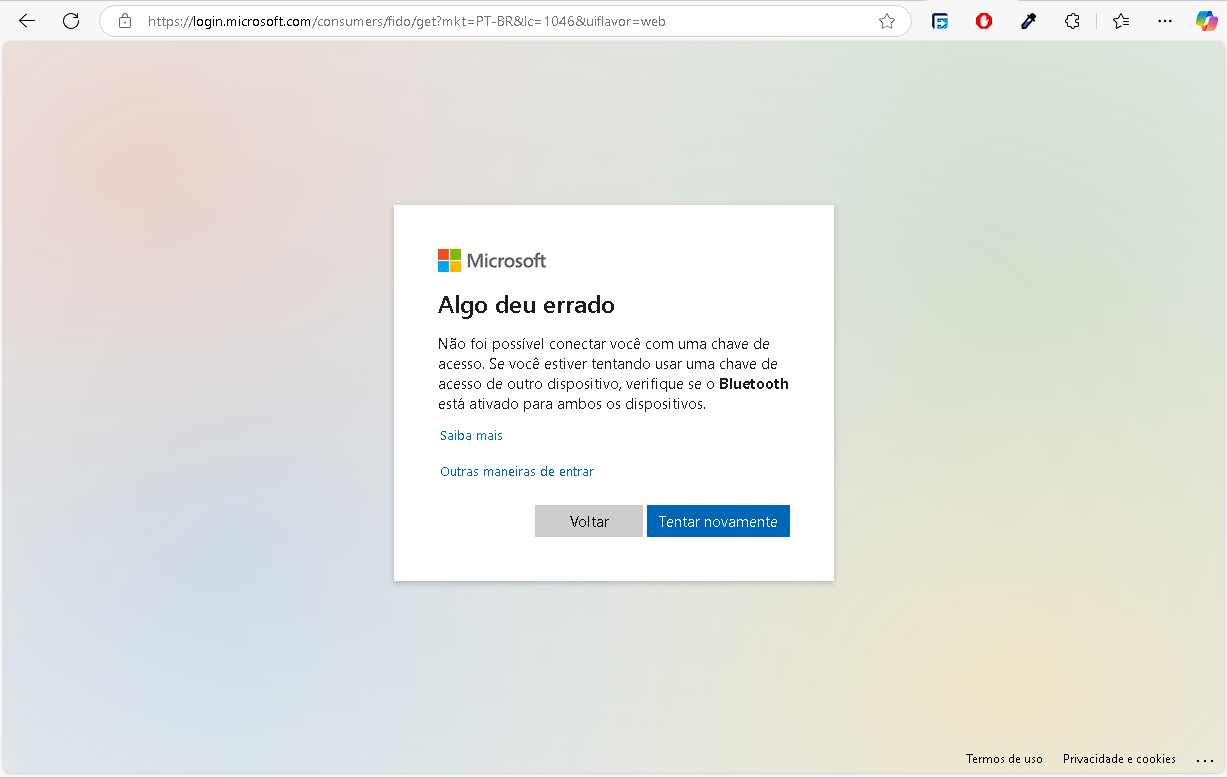
\includegraphics[width=0.7\textwidth]{./assets/microsoft_error_2.png}
  \caption{Erro no duplo fator de autenticação da Microsoft}
  \label{fig:Microsoft2FactoryAutenticatorError}
\end{figure}

\subsubsection{Aegis}

Já o Aegis, por ser um aplicativo de código aberto, oferece maior transparência
e controle sobre os dados do usuário, mas possui uma interface de configuração
e arquivos que pode ser menos amigável para usuários mais leigos.
Nele é possível adicionar e gerenciar chaves de autenticação de dois fatos,
exportar e importar cópias de segurançats para diversos aplicativos ou em formato de arquivos,
inclusive em formato criptografado.

A maior vantagem do Aegis é a possibilidade de instalar o aplicativo por meio da
loja de aplicativos de código aberto F-Droid, uma alternativa ao Google Play
Store, permitindo que o mesmo possa ser intalado em dispositivos Android sem GMS
ou AOSP (Android \textit{Open Source Project}).
Vale destacar que o aplicativo tem instruções de recomendações e avisos para lembrar o usuário
de realizar cópias de segurança e mais.

\subsection{Avaliação de Aplicativos de Gerenciamento de Senhas}

No sistema operacional Android com GMS o Google automaticamente oferece um popup
para salvar a senha no momento em que é digitada no processo de autenticação de
algum aplicativo ou serviço.
Como o Google não é especificamente um aplicativo de segurança, pode parecer um
pouco escondido a opção de gerenciar as senhas pelas configurações de conta.
Além do gerenciamento de senhas com sincronização em nuvem, é possível adicionar
anotações, exportar e importar em formato de planilha CSV sem criptografia.

O mesmo pop-up do Android utilizado pelo Google pode ser substituido por
aplicativos de terceiros, como o Microsoft Authenticator, citado anteriormente
que oferece recursos adicionais para gerenciar senhas.
Também permite adicionar anotações, exportar e importar em formato de planilha
CSV sem criptografia.

No sistema operacional Windows não há opção nativa ou pré instalada para
salvar senhas, dependendo de programas de terceiros para salvar senhas.
Navegadores de internet normalmente oferecem uma opção nativa para salvar senhas,
mas com poucos recursos extras de segurança ou gerenciamento.
Infelismente os navegadores de internet não solicitam uma senha mestre para liberar
a autenticação ou até mesmo para visualizar a senha.

\subsubsection{KeePass}

O KeePass é um aplicativo ou programa de código aberto para computadores pessoais.
Diferente dos aplicativos citados anteriormente, o KeePass não é um aplicativo
para dispositivos móveis como tablets ou \textit{smartphone}, mas sim um aplicativo desktop,
que pode ser instalado em qualquer dispositivo com sistema operacional Windows.
Existem também versões para outros sistemas operacionais como Linux, Mac OS e até
BSD, desenvolvido por contribuidores não oficiais.

A figura \ref{fig:KeePass} mostra a interface do KeePass, por padrão o ele é em inglês,
necessitando de plugins de tradução para outras idiomas.
Embora a interface aparente ser para computadores mais antigos, não se trata de um
aplicativo desatualizado, mas sim um aplicativo com uma interface única, compatível
com qualquer sistema operacional recente.
Além de que a interface é amigável para gerenciar senhas, com maior foco no gerenciamento
das anotações e com sugestões inteligentes de senhas fortes.

KeePass não tem integração com o sistema operacional, ou seja, nele, o usuário vai apenas
realizar anotações, sem possibilidade de auto completar senhas em processos de autenticação
e sem sincronização com outros dispositivos.
O KeePass permite salvar as senhas em formato de arquivos com criptografia, os arquivos
são salvos localmente pelo qual o usuário deve se compromenter em salvar em um local
seguro e manter cópias de segurança em outros locais.
Entretanto, o próprio aplicativo oferece e sugere a possibilidade de imprimir uma cópia
de segurança do arquivo de senhas.

\begin{figure}[h!]
  \centering
  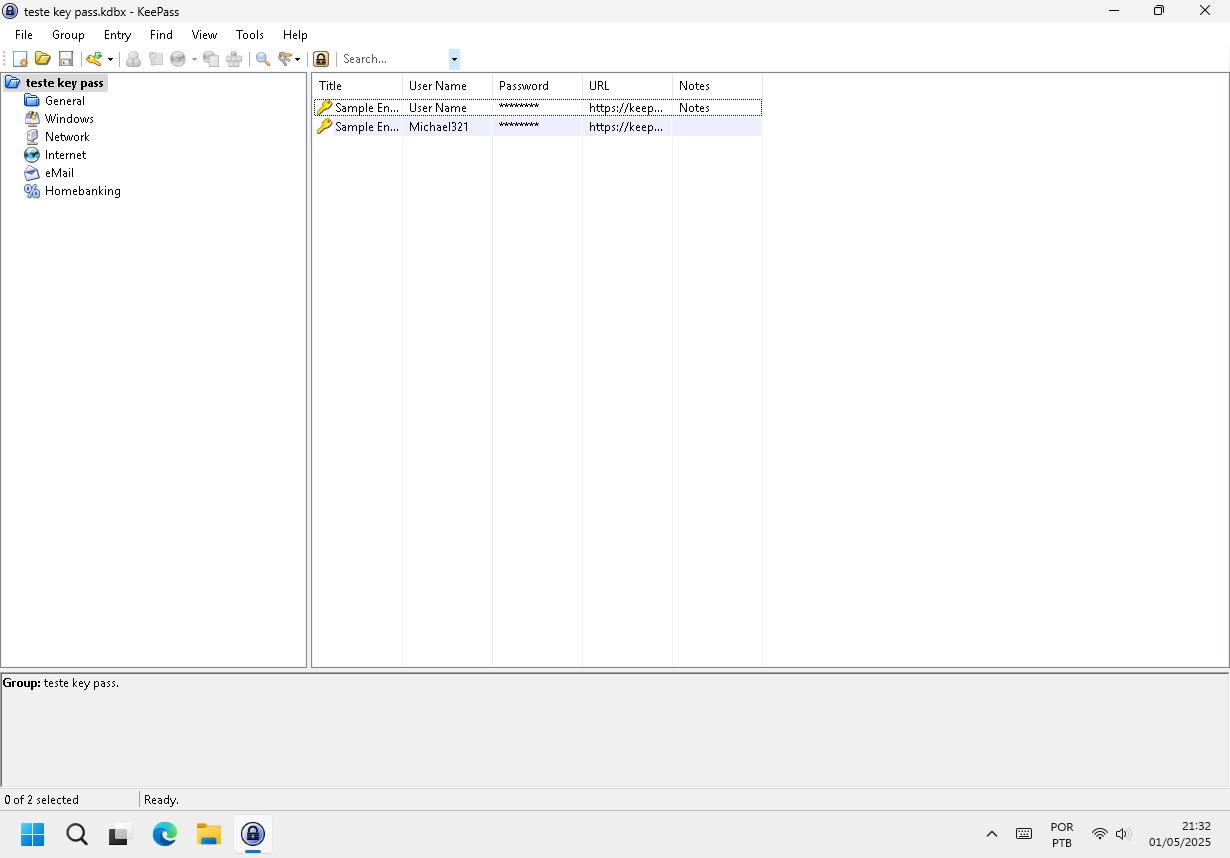
\includegraphics[width=0.7\textwidth]{./assets/keepass.png}
  \caption{Programa de gerenciamento de senhas KeePass}
  \label{fig:KeePass}
\end{figure}

\subsubsection{KeeWeb}

No site oficial de KeePass exístem vários aplicativos que são contribuições não oficiais
de KeePass, como KeeWeb que é um aplicativo de código aberto compatível com KeePass, em
que é possível utilizar o mesmo banco de dados do KeePass.
Diferente dos aplicativos citados anteriormente, o KeeWeb não é um aplicativo
nativo, mas sim um aplicativo web progressivo, multi plataforma, que pode ser instalado
em qualquer dispositivo com navegador de internet.
Assim como KeePass, não há integração com o sistema operacional para auto completar senhas
em processo de autenticação.

A figura \ref{fig:KeeWeb} apresenta o aplicativo KeeWeb.
Por padrão o a tradução do aplicativo é em inglês, também necessitando de plugins de
tradução para outros idiomas, entretanto com a praticidade de poder instalar os plugins
diretamente pelo aplicativo.
O KeeWeb apresenta uma interface moderna e amigável para gerenciar senhas, com o mesmo foco
no gerenciamento das anotações assim como no KeePass, com a diferença de que o KeeWeb
permite salvar as anotações de senhas com ou sem criptografia, onde os arquivos ficam
dentro da memoria do navegador de internet e podem ser exportados localmente em formato de
arquivos.

Há um diferencial nesse aplicativo que permite exportar os arquivos em nuvens de serviços
de terceiros em que o usuários tiver preferencia.
Utilizar aplicativos de gerenciamento de senhas, apresentou grande praticidade,
especialmente para os serviços que não se mantem autenticados, solicitam a
autenticação com frequencia ou perdem a autenticação por defeito.

Porém os aplicativos de gerenciamento de senhas e navegadores de internet não
são perfeitos, em alguns casos, apresnetam o popup sob a caixa de entrada do
login, senha ou botões.
Já o KeeWeb, quando não configurado para o mesmo idioma do dispositivo, é
prejudicado no sistema operacional Android, por ser um aplicativo web progressivo,
o Google Chrome insiste em traduzir o aplicativo e até mesmo as senhas, tornando
as senhas inválidas.

\begin{figure}[h!]
  \centering
  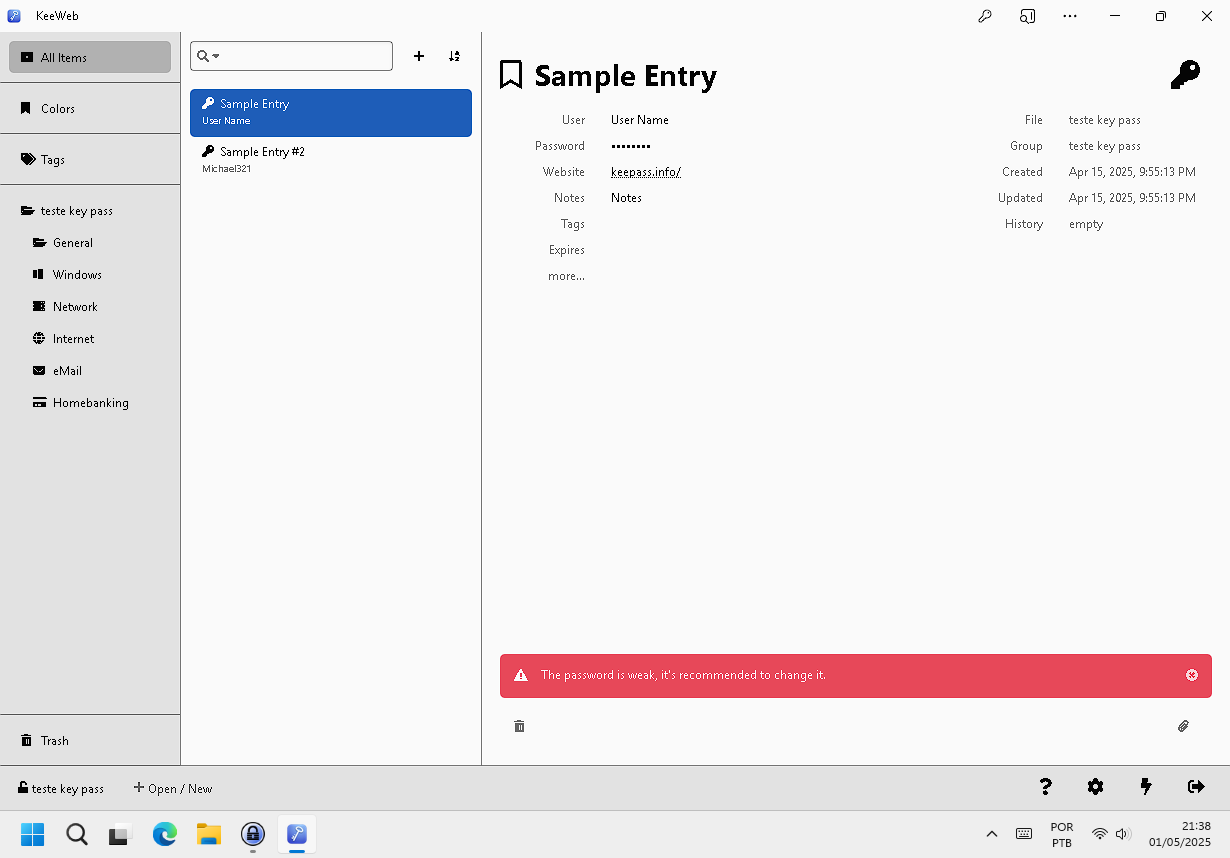
\includegraphics[width=0.7\textwidth]{./assets/keeweb.png}
  \caption{Aplicativo de gerenciamento de senhas KeeWeb}
  \label{fig:KeeWeb}
\end{figure}

\section{Considerações Finais}

% \subsection{Resultados do quesstionário}

A pesquisa revela que, embora a maioria dos entrevistados utilize algum tipo de multi fator
de autenticação e tenha uma percepção boa da segurança dos serviços, ainda há espaço para
melhoria, podendo aprimorar ainda mais a força das senhas, adotar práticas para anotar as
credenciais ao invéz de memoriza-las e priorizar o uso de duplo fator de autenticação, tais
como códigos OTP, evitando especialmente as verificações via SMS.
Os incidentes de segurança relatados por uma parcela significativa dos participantes
reforçam a importância de práticas de segurança digital mais robustas e da
conscientização sobre os riscos.
A sugestão de um entrevistado sobre o uso de dados falsos destaca uma preocupação
com a privacidade que pode influenciar o comportamento do usuário em relação à
segurança.

% \subsection{Resultados de Programas e Aplicativos}

O duplo fator de autenticação baseado em OTP adiciona uma camada extra de segurança
para proteger as contas dos usuários.
Dos aplicativos móveis testados, o Google Authenticator foi o mais simples de usar,
enquanto que o Aegis apresentou maior compatibilidade com diferentes dispositivos e
o Microsoft Authenticator foi o mais completo, porém com diversas instabilidades.
No entanto, nem todos os serviços digitais são compatíveis com duplo fator de
autenticação baseados em OTP, além de que tal tecnologia tende a ser restrita a
dispositivos móveis e chaves físicas.

Memorizar múltiplas credenciais de acesso, especialmente aquelas com senhas de alta
entropia, é improvável para a maioria das pessoas.
Optar por realizar anotações em um caderno, reduz os desafios tecnológicos, mas
demanda atenção especial ao registrar caracteres especiais, letras maiúsculas e
minúsculas, evitando erros.

Armazenar informações de senhas e credenciais de acesso em meio digital oferece mais
praticidade, mas exige conhecimento técnico, uso de programas ou aplicativos de
terceiros e cuidados com a segurança do local de armazenamento dos dados.
Embora os navegadores de internet e alguns sistemas operacionais ofereçam opções
nativas para armazenar senhas, programas e aplicativos testados, como KeePass e KeeWeb
oferecem maior rigor na segurança e flexibilidade na gestão de informações.

Embora existam diversas opções de aplicativos e programas voltados à segurança
pessoal, a escolha da ferramenta mais adequada para uso individual não é tão
simples, pois a complexidade técnica e a experimentação pode representar um obstáculo.
Importante ressaltar que é essencial realizar cópias de segurança para evitar
complicações, tanto para as chaves de duplo fator de autenticação baseado em OTP,
quanto as anotações de senhas e credenciais de acesso, porém nem todos os programas,
aplicativos ou serviços digitais reforçam essa prática.

Independentemente de como o usuário armazene suas credenciais, é essencial evitar o
registro de senhas em locais inapropriados, como aplicativos de bloco de notas,
mensagens instantâneas ou até na agenda de contatos do telefone.
Esses recursos não são criptografados e, por não terem sido desenvolvidos para esse
propósito, tornam-se vulneráveis à exploração por usuários mal-intencionados ou a falhas
de segurança.

% \subsection{Considerações Sobre a Segurança}

Por mais sofisticados que os serviços digitais possam ser, não existe garantias de segurança.
Cada estratégia de segurança é uma camada a mais, uma barreira adicionado contra ataques.
Ao mesmo tempo, cada camada adiciona complexidade, necessitando de anotações, cópias de
segurança e até aplicativos confiaveis, do contrário, as camadas de segurança que deviam
proteger o usuário, pode se tornar um obstáculo para o próprio usuário.

A conscientização sobre golpes é crucial, pois o conhecimento é a primeira linha de defesa contra
os ataques cibernéticos.
É importante estar atento a mensagens e propagandas que possam ser enganosas, solicitando dados
confidênciais ou fornecendo algo suspeito.
Ao receber um código de autenticação sem solicitar, não o informe a ninguém e altere a senha,
pois pode ser uma tentativa de invasão.

Todo o serviço que é bem feito, vai usar um algoritmo de derivação de chave e nunca vai salvar
as senhas das credenciais de forma aberta.
Logo, se o mesmo limita o comprimento ou variabilidade de caracteres do cadastro da senha, é um
grande indicativo de que o serviço não está preocupado com a segurança dos dados dos usuários.
Mesmo assim, senhas devem ter alta entropia, ou seja, devem ser longas e misturar todas as opções
digitáveis do teclado, pois a senha é a primeira barreira de segurança.

\bibliographystyle{sbc}
\bibliography{references}

\end{document}